\documentclass{../cscslides}

\slidetitle{Лекция 4: Моделирование и анализ}{28.02.2022}

\begin{document}

    \frame{\titlepage}

    \section{Моделирование требований}

    \begin{frame}
        \frametitle{Моделирование требований}
        Первый этап разработки любой системы --- сбор и анализ требований
        \begin{itemize}
            \item Понимание разработчиками решаемой задачи
            \item Соглашение между разработчиками, заказчиками и пользователями
            \begin{itemize}
                \item Заказчики и пользователи часто разные люди с разными потребностями
            \end{itemize}
            \item Чёткое обозначение границ системы
            \item Основа для планирования проекта
            \item Чаще всего словесное описание требований, реже формальные модели
        \end{itemize}
    \end{frame}

    \section{Моделирование случаев использования}
    
    \begin{frame}
        \frametitle{Диаграмма случаев использования UML}
        \framesubtitle{Диаграмма прецедентов}
        \begin{columns}
            \begin{column}{0.5\textwidth}
                \begin{itemize}
                    \item Ивар Якобсон, 1992 год
                    \item Акторы (или актёры, роли) --- внешние сущности, использующие систему
                    \begin{itemize}
                        \item Люди или другие программные системы
                    \end{itemize}
                    \item Случаи использования (прецеденты)  --- цель использования системы актором
                    \begin{itemize}
                        \item Раскрываются в набор сценариев, описываемых чаще текстом
                    \end{itemize}
                \end{itemize}
            \end{column}
            \begin{column}{0.5\textwidth}
                \begin{center}
                    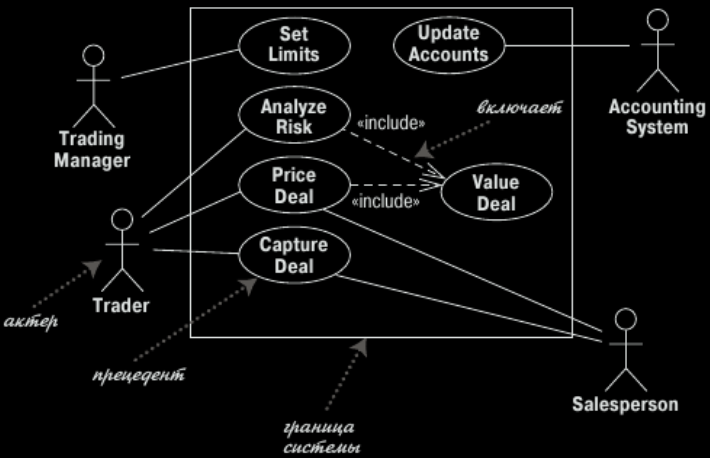
\includegraphics[width=\textwidth]{useCaseDiagramBlack.png}
                    \attribution{М. Фаулер, UML. Основы}
                \end{center}
            \end{column}
        \end{columns}
    \end{frame}

    \begin{frame}
        \frametitle{Include и Extend}
        Include:
        \begin{center}
            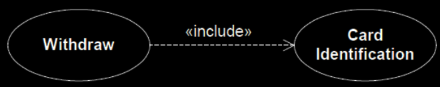
\includegraphics[width=0.45\textwidth]{useCaseIncludeBlack.png}
        \end{center}
        \vspace{5mm}
        Extend:
        \begin{center}
            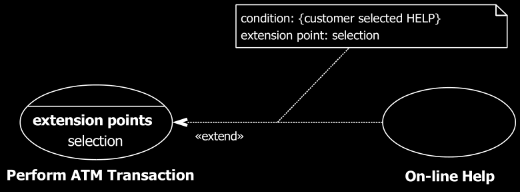
\includegraphics[width=0.5\textwidth]{useCaseExtendBlack.png}
        \end{center}
        \attribution{OMG, UML 2.5 Specification}
    \end{frame}

    \begin{frame}
        \frametitle{Пример, check-in в аэропорту}
        \begin{center}
            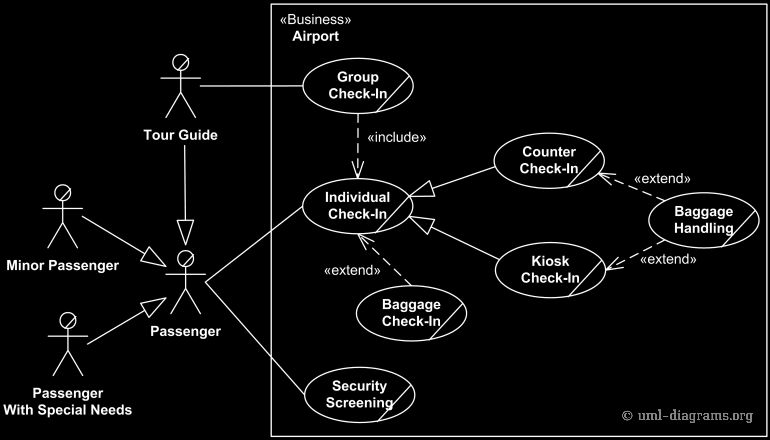
\includegraphics[width=0.7\textwidth]{airportUseCaseBlack.png}
            \attribution{http://www.uml-diagrams.org}
        \end{center}
    \end{frame}

    \begin{frame}
        \frametitle{Сценарий использования, типичная структура}
        \begin{itemize}
            \item Заголовок (цель основного актора)
            \item Заинтересованые лица, акторы, основной актор
            \item Предусловия
            \item Триггеры (активаторы)
            \item Основной порядок событий
            \item Альтернативные пути и расширения
            \item Постусловия
        \end{itemize}
    \end{frame}

    \begin{frame}
        \begin{center}
            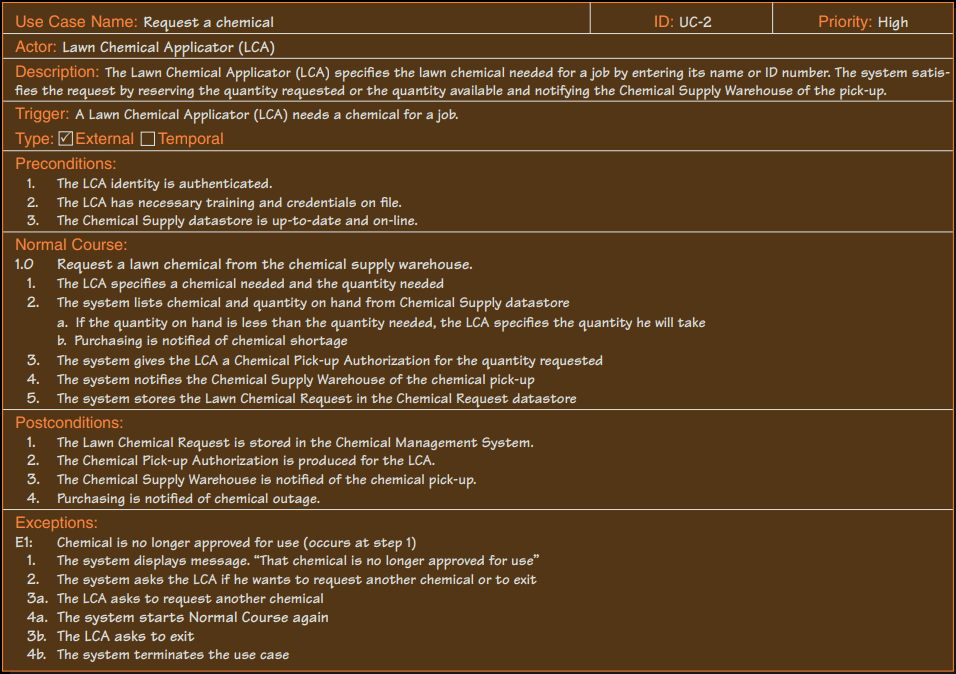
\includegraphics[width=0.9\textwidth]{useCaseExampleBlack.png}
            \attribution{R.M. Roth et al., System Analysis and Design}
        \end{center}
    \end{frame}

    \section{IDEF0}

    \begin{frame}
        \frametitle{Контекстная диаграмма IDEF0}
        \begin{itemize}
            \item Обозначает границы системы и способы её взаимодействия с внешним миром
            \item Используется для моделирования не только ПО
            \item Каждая сторона имеет свой смысл
            \begin{itemize}
                \item Слева --- входные данные или материалы
                \item Сверху --- управление
                \item Снизу --- механизмы
                \item Справа --- выходные данные или продукты
            \end{itemize}
        \end{itemize}
        \begin{center}
            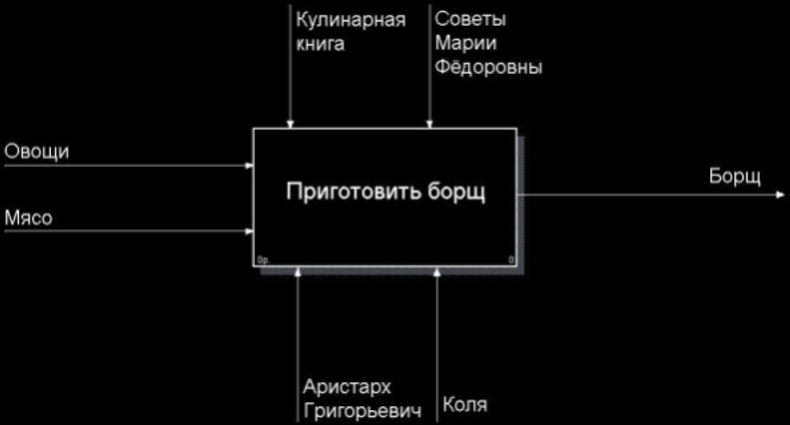
\includegraphics[width=0.4\textwidth]{idef0ExampleBlack.png}
            \attribution{http://ecm-journal.ru}
        \end{center}
    \end{frame}

    \section{Моделирование характеристик}

    \begin{frame}
        \frametitle{Диаграмма характеристик}
        \framesubtitle{Feature Diagram}
        \begin{itemize}
            \item Представляет функциональность системы в виде дерева
            \item Используется в основном для моделирования семейств программных продуктов (Product lines)
        \end{itemize}
        \begin{center}
            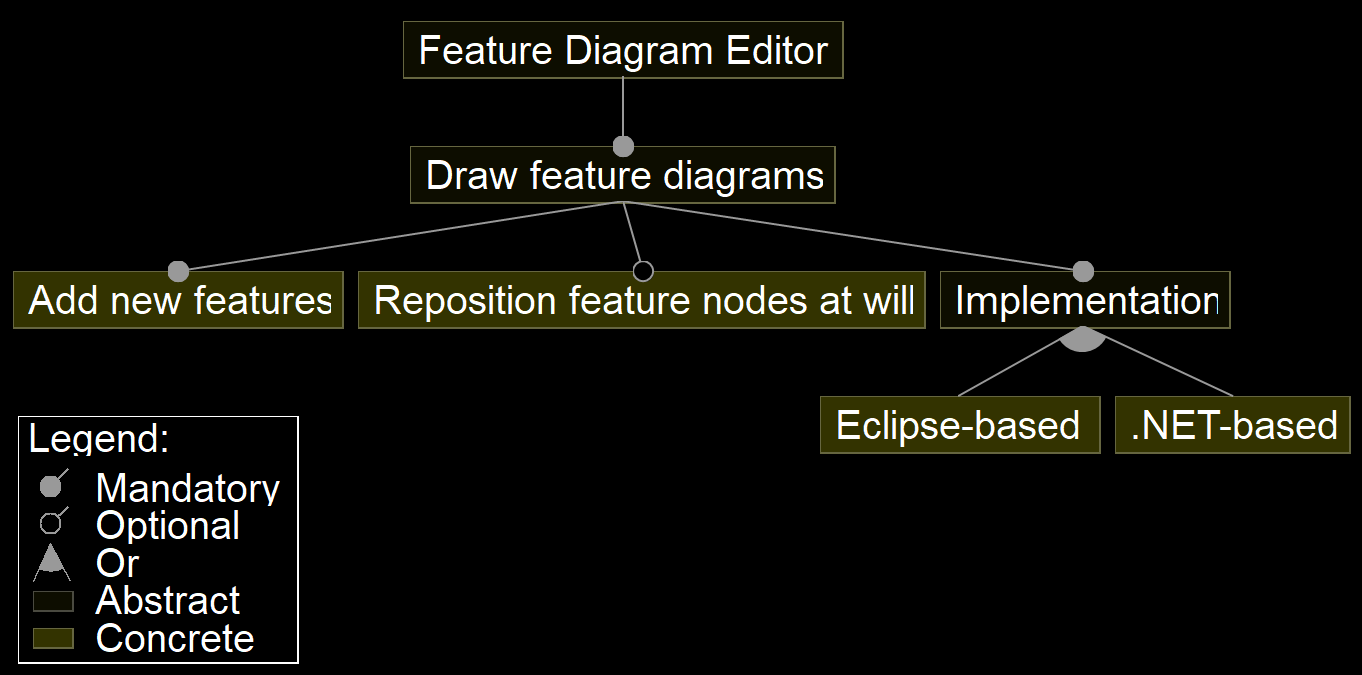
\includegraphics[width=0.6\textwidth]{featureDiagramBlack.png}
        \end{center}
    \end{frame}

    \begin{frame}
        \frametitle{Диаграмма характеристик, пример}
        \begin{center}
            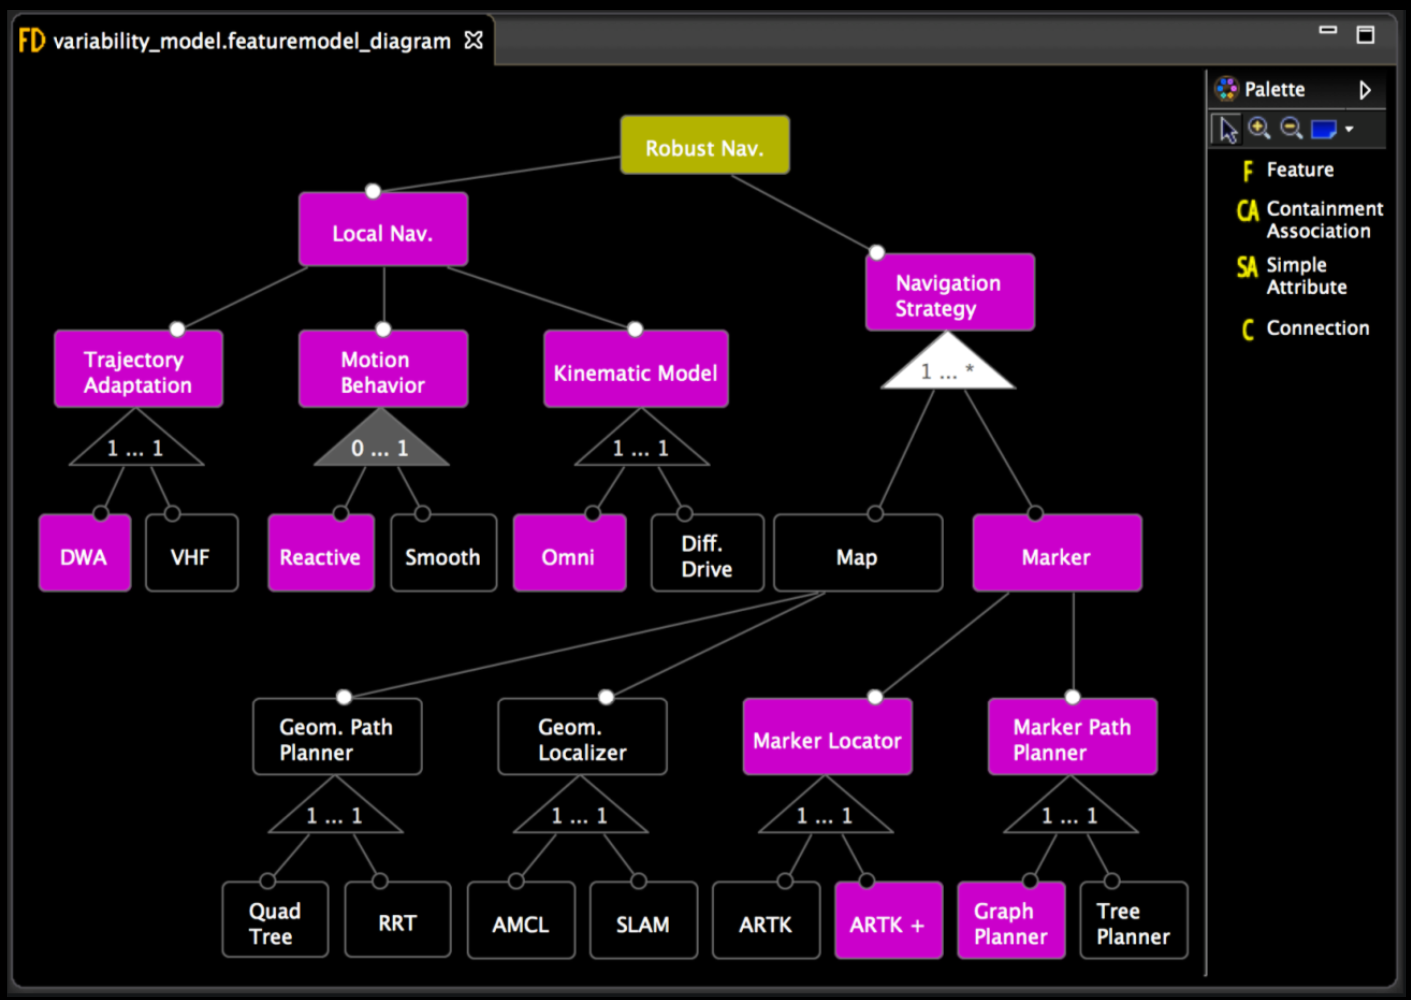
\includegraphics[width=0.8\textwidth]{featureDiagramExampleBlack.png}
            \attribution{D. Brugali}
        \end{center}
    \end{frame}

    \begin{frame}
        \frametitle{Feature Tree}
        \begin{center}
            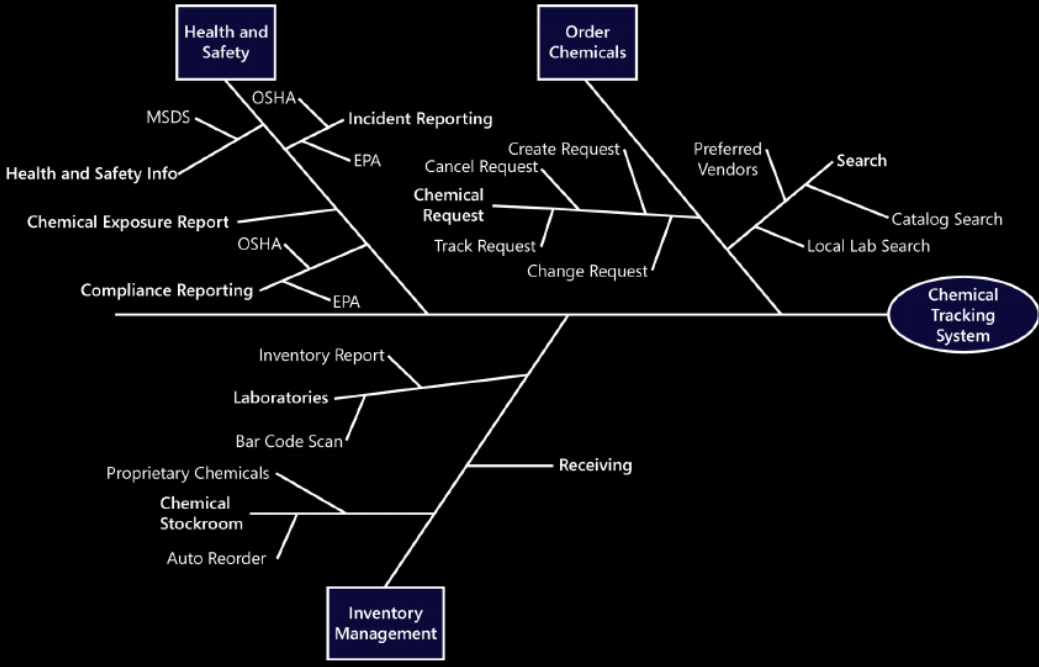
\includegraphics[width=0.8\textwidth]{featureTreeBlack.png}
        \end{center}
    \end{frame}

    \section{Моделирование требований в SysML}

    \begin{frame}
        \frametitle{Диаграмма требований, SysML}
        \begin{itemize}
            \item Более формальная нотация дерева фич
        \end{itemize}
        \begin{center}
            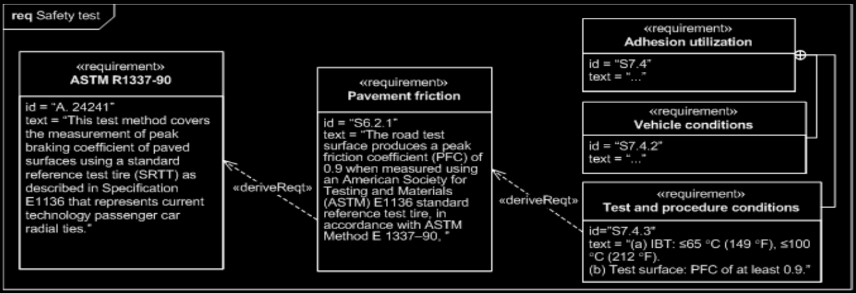
\includegraphics[width=0.6\textwidth]{sysMlRequirementDiagramBlack.png}
            \attribution{OMG SysML 1.4 Specification}
        \end{center}
    \end{frame}

    \begin{frame}
        \frametitle{Диаграмма требований SysML, пример}
        \begin{center}
            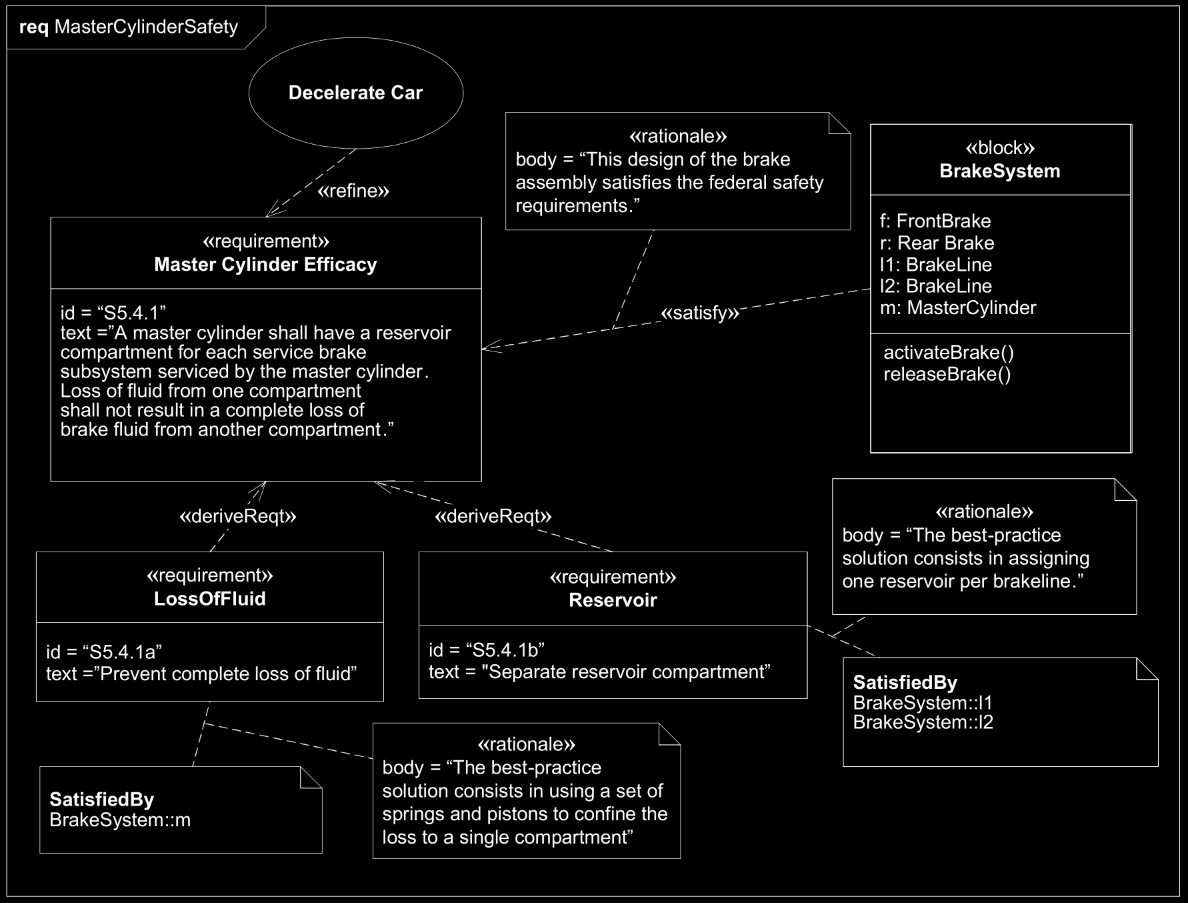
\includegraphics[width=0.75\textwidth]{sysMlRequirementsExampleBlack.png}
            \attribution{OMG SysML 1.4 Specification}
        \end{center}
    \end{frame}

    \begin{frame}
        \frametitle{Диаграмма требований SysML и тесты}
        \begin{columns}
            \begin{column}{0.5\textwidth}
                Требования:
                \begin{center}
                    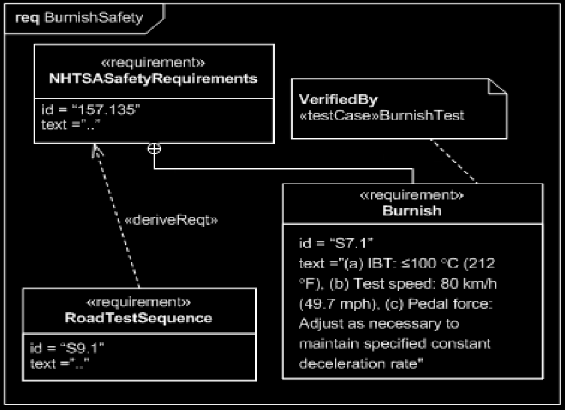
\includegraphics[width=0.8\textwidth]{sysMlRequirementsTestBlack.png}
                \end{center}
            \end{column}
            \begin{column}{0.5\textwidth}
                Сценарий тестирования:
                \begin{center}
                    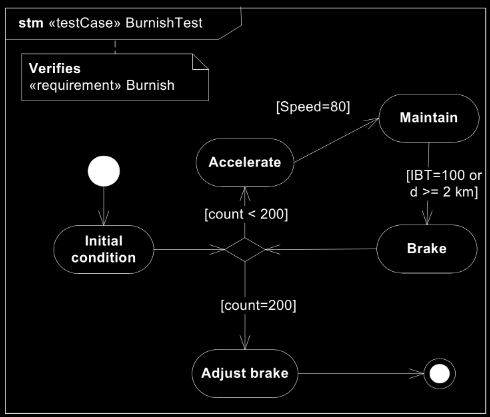
\includegraphics[width=0.9\textwidth]{sysMlRequirementsTestActivityBlack.png}
                    \attribution{OMG SysML 1.4 Specification}
                \end{center}
            \end{column}
        \end{columns}
    \end{frame}

    \section{Диаграмма активностей UML}

    \begin{frame}
        \frametitle{Диаграмма активностей UML}
        \framesubtitle{Диаграммы деятельности}
        \begin{columns}
            \begin{column}{0.5\textwidth}
                \begin{itemize}
                    \item Используются для моделирования бизнес-процессов, тоже на первых этапах
                    \begin{itemize}
                        \item Может быть визуализацией сценария использования
                    \end{itemize}
                    \item Иногда --- для моделирования алгоритма
                    \item Расширенные блок-схемы
                    \item Семантика на основе сетей Петри
                \end{itemize}
            \end{column}
            \begin{column}{0.5\textwidth}
                \begin{center}
                    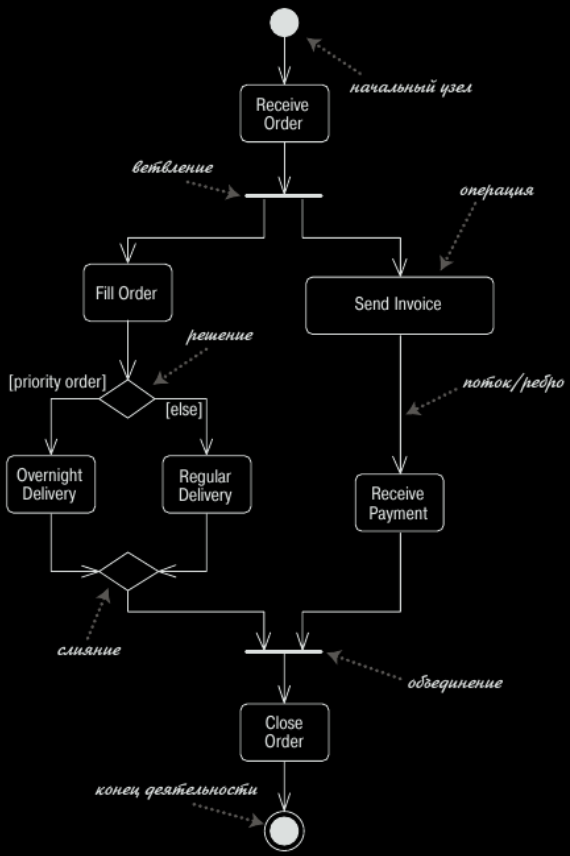
\includegraphics[width=0.7\textwidth]{activityDiagramBlack.png}
                    \attribution{М. Фаулер, UML. Основы}
                \end{center}
            \end{column}
        \end{columns}
    \end{frame}

    \begin{frame}
        \frametitle{Диаграмма активностей, разделы}
        \begin{columns}
            \begin{column}{0.5\textwidth}
                \begin{itemize}
                    \item Раздел представляет отдел организации (или организацию), отвечающий за часть работы
                    \item Визуализирует поток работ между отделами
                \end{itemize}
            \end{column}
            \begin{column}{0.5\textwidth}
                \begin{center}
                    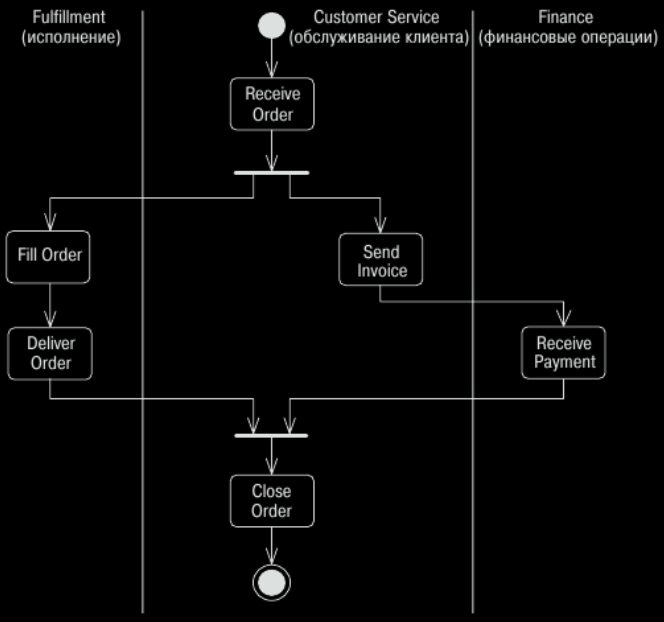
\includegraphics[width=0.9\textwidth]{activitySwimlanesBlack.png}
                    \attribution{М. Фаулер, UML. Основы}
                \end{center}
            \end{column}
        \end{columns}
    \end{frame}

    \begin{frame}
        \frametitle{Диаграмма активностей, сигналы}
        \begin{itemize}
            \item Для визуализации асинхронных процессов
            \item Сигналом может быть посылка документа, запрос и т.д.
        \end{itemize}
        \begin{center}
            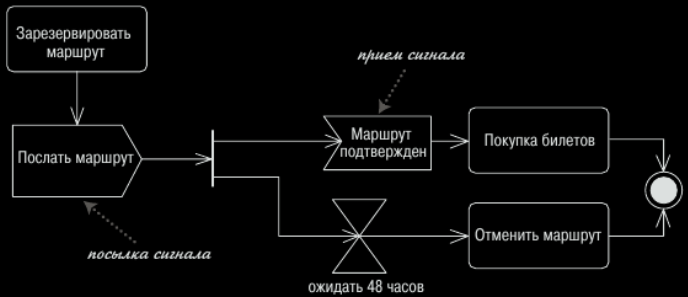
\includegraphics[width=0.6\textwidth]{activitySignalsBlack.png}
            \attribution{М. Фаулер, UML. Основы}
        \end{center}
    \end{frame}

    \section{BPMN}

    \begin{frame}
        \frametitle{Business Process Model and Notation}
        \begin{itemize}
            \item Версия 1.0 в 2004 году, текущая (2.0) --- в 2011
            \item Для описания бизнес-процессов
            \begin{itemize}
                \item Сильно продвинутые диаграммы активностей
                \item Позволяют описывать группы взаимодействующих процессов
                \item Исполнимая семантика
                \item Правила генерации в BPEL
                \begin{itemize}
                    \item Business Process Execution Language
                \end{itemize}
            \end{itemize}
        \end{itemize}
    \end{frame}

    \begin{frame}
        \frametitle{Пример диаграммы}
        \begin{center}
            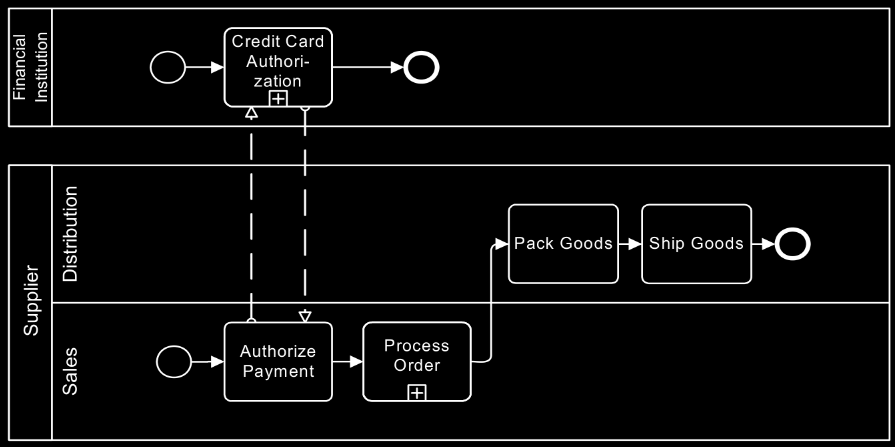
\includegraphics[width=0.9\textwidth]{bpmnExampleBlack.png}
            \attribution{OMG BPMN 2.0 Specification}
        \end{center}
    \end{frame}

    \begin{frame}
        \frametitle{События}
        \begin{center}
            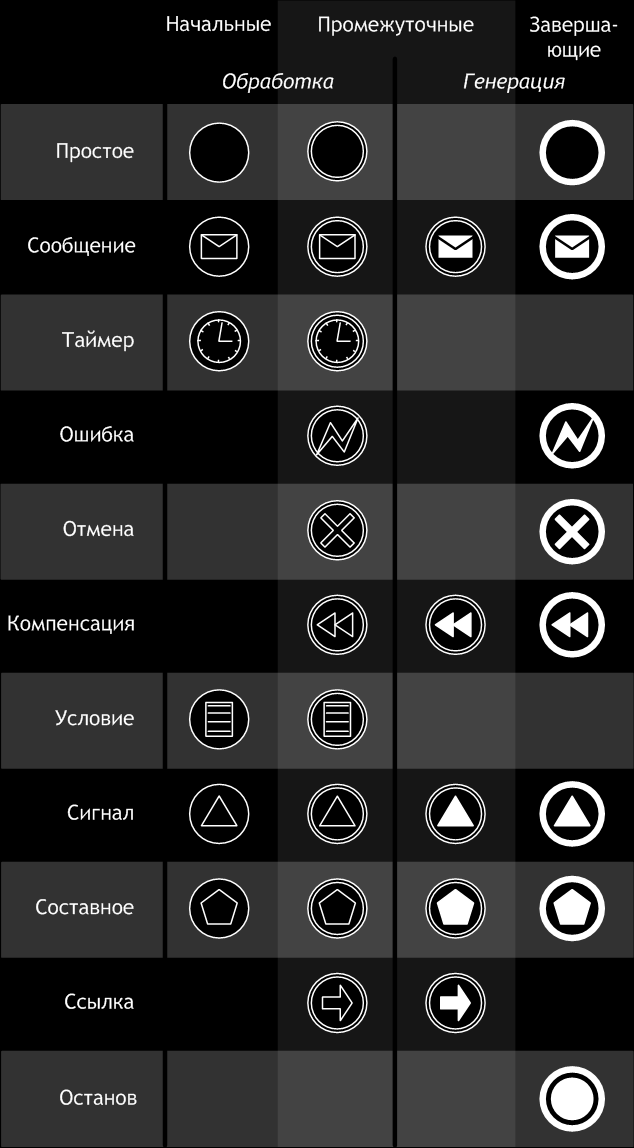
\includegraphics[height=0.8\textheight]{bpmnEventsBlack.png}
            \attribution{\url{https://ru.wikipedia.org/wiki/BPMN}}
        \end{center}
    \end{frame}

    \begin{frame}
        \frametitle{Операторы ветвления}
        \begin{center}
            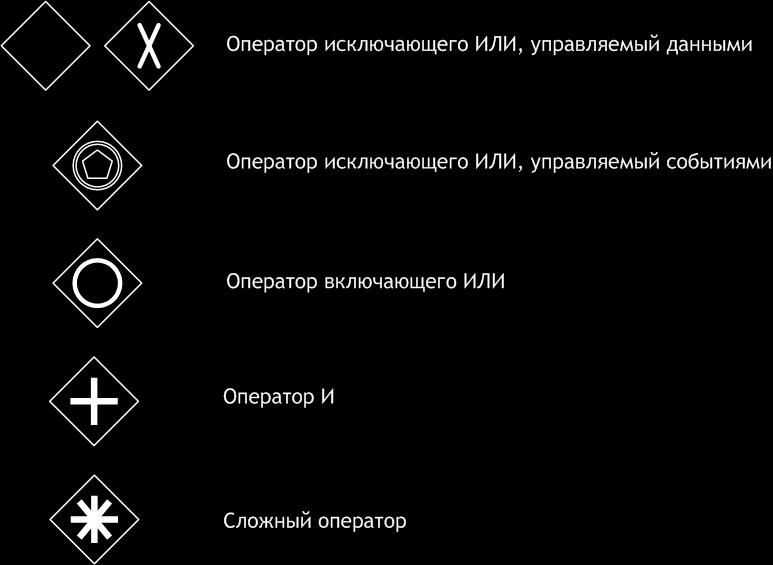
\includegraphics[width=0.5\textwidth]{bpmnGatewaysBlack.png}
            \attribution{\url{https://ru.wikipedia.org/wiki/BPMN}}
        \end{center}
    \end{frame}

    \begin{frame}
        \frametitle{Диаграмма хореографии}
        \begin{center}
            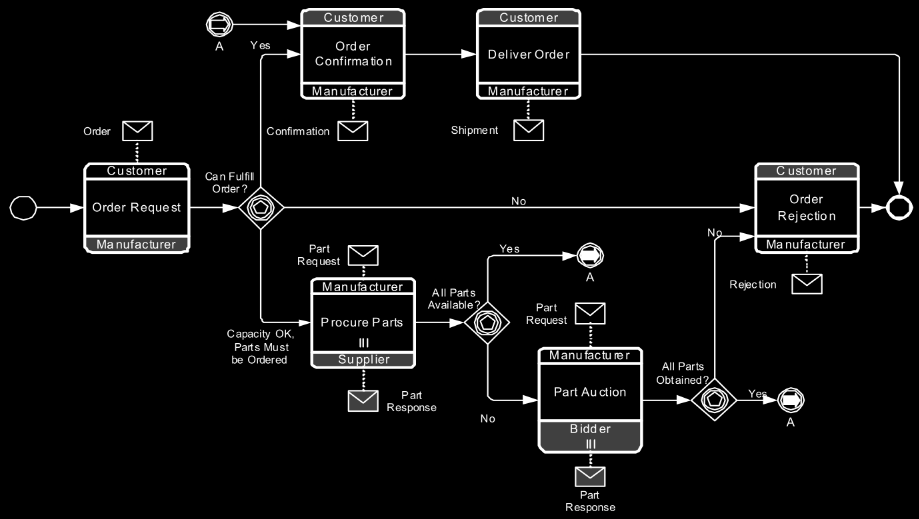
\includegraphics[width=0.9\textwidth]{bpmnChoreographyBlack.png}
            \attribution{OMG BPMN 2.0 Specification}
        \end{center}
    \end{frame}

    \begin{frame}
        \frametitle{Диаграмма диалогов}
        \begin{center}
            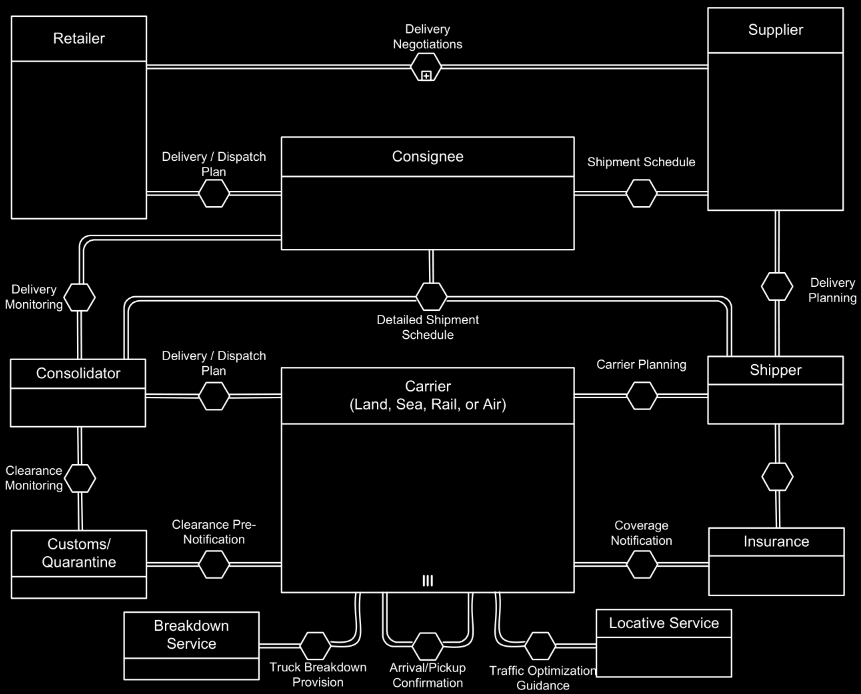
\includegraphics[width=0.7\textwidth]{bpmnConversationBlack.png}
            \attribution{OMG BPMN 2.0 Specification}
        \end{center}
    \end{frame}

    \section{Диаграмма развёртывания}
    
    \begin{frame}
        \frametitle{Диаграмма развёртывания UML}
        \begin{columns}
            \begin{column}{0.5\textwidth}
                \begin{itemize}
                    \item Показывает отображение компонентов и физических артефактов на реальные (или виртуальные) устройства
                    \item Бывает полезна на начальных этапах проектирования, даже до диаграмм компонентов
                \end{itemize}
            \end{column}
            \begin{column}{0.5\textwidth}
                \begin{center}
                    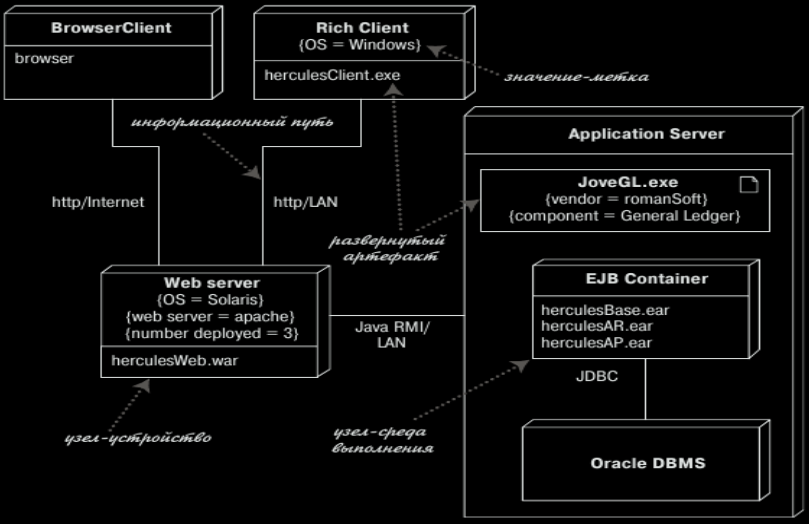
\includegraphics[width=\textwidth]{deploymentDiagramBlack.png}
                    \attribution{М. Фаулер, UML. Основы}
                \end{center}
            \end{column}
        \end{columns}
    \end{frame}

    \section{Диаграммы ``Сущность-связь''}

    \begin{frame}
        \frametitle{Диаграммы ``Сущность-связь''}
        \begin{columns}
            \begin{column}{0.5\textwidth}
                \begin{itemize}
                    \item Описывают концептуальную модель предметной области
                    \item Идеальны для моделирования схем реляционных баз данных
                    \item 1976 год, Питер Чен
                \end{itemize}
            \end{column}
            \begin{column}{0.5\textwidth}
                \begin{center}
                    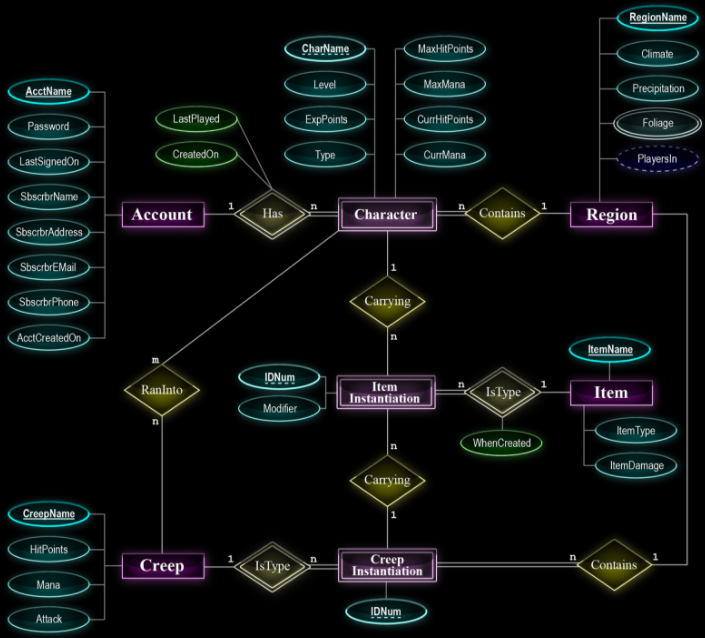
\includegraphics[width=\textwidth]{erChenNotationBlack.png}
                    \attribution{https://ru.wikipedia.org}
                \end{center}
            \end{column}
        \end{columns}
    \end{frame}

    \begin{frame}
        \frametitle{Нотация ``Вороньей лапки''}
        \begin{center}
            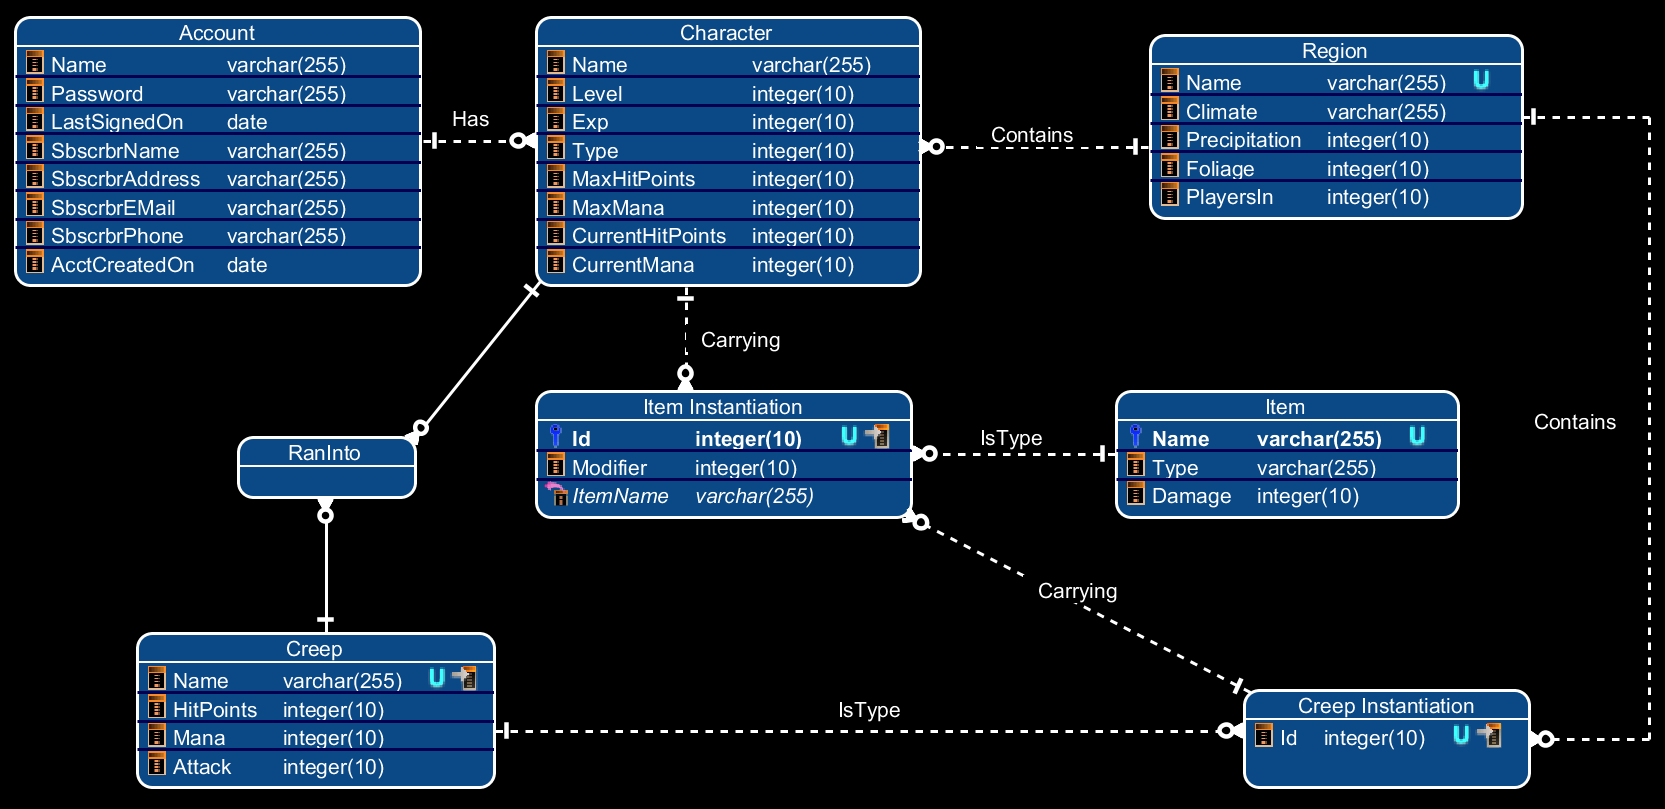
\includegraphics[width=\textwidth]{erCrowsFootBlack.png}
        \end{center}
    \end{frame}

    \section{Диаграммы ORM}
    
    \begin{frame}
        \frametitle{Object-Role Modeling}
        \begin{center}
            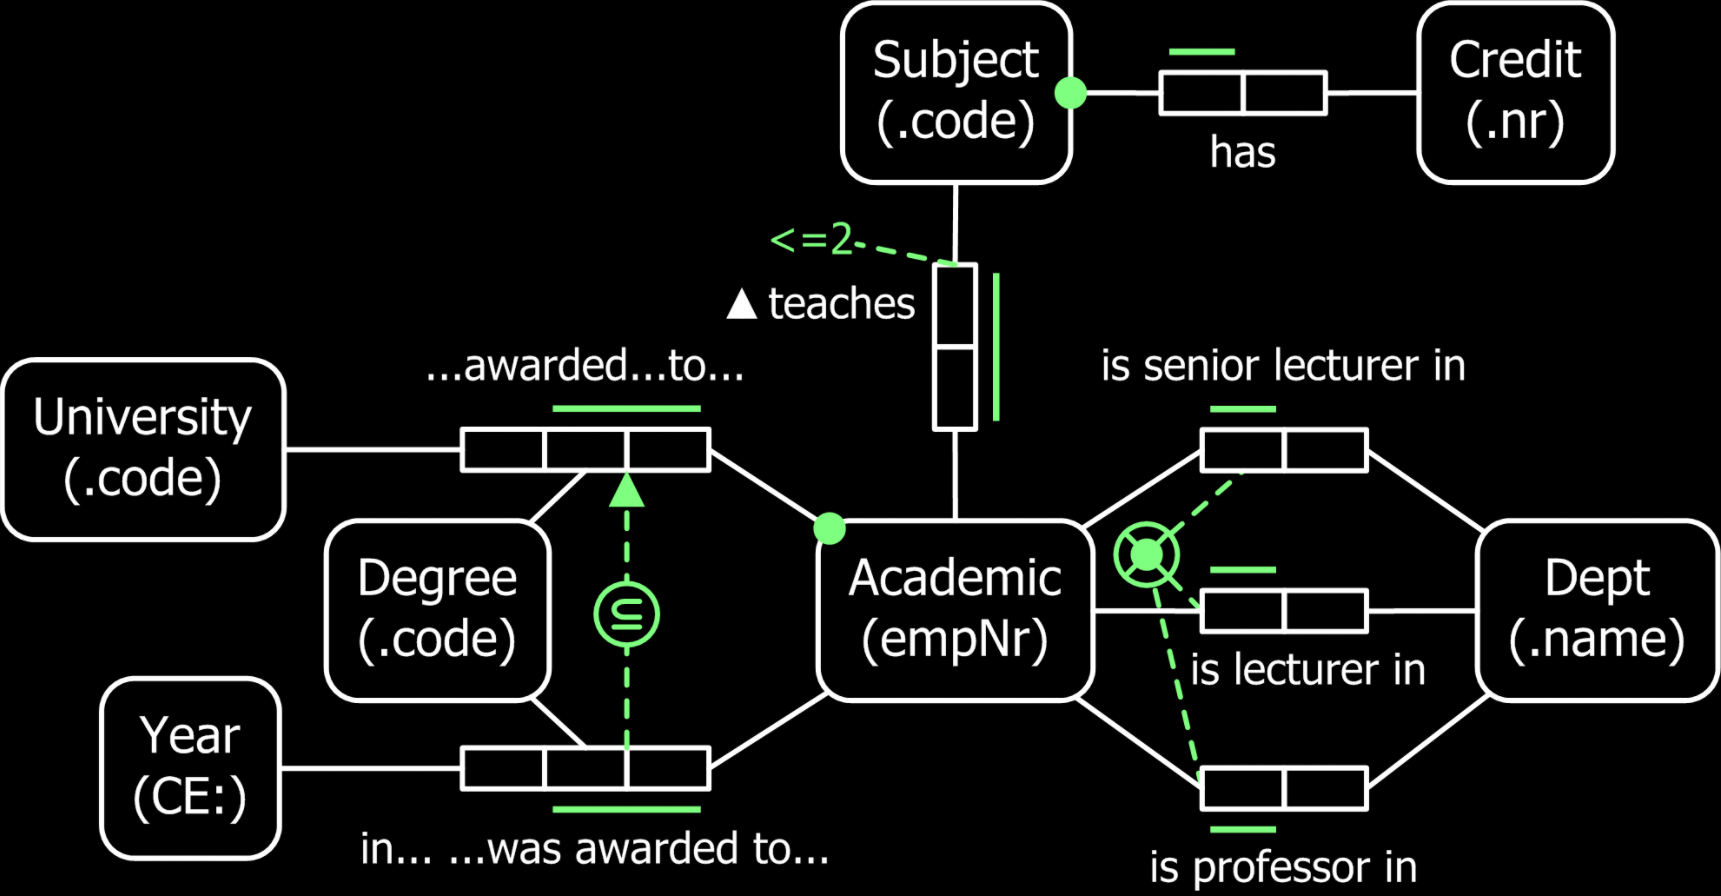
\includegraphics[width=0.8\textwidth]{ormBlack.png}
            \attribution{http://www.orm.net}
        \end{center}
    \end{frame}

\end{document}
